\documentclass[../../main.tex]{subfiles}

\begin{document}

\section{LabView III}

\begin{fulltheorem}
  A LabVIEW programnyelv struktúrái, programozási lehetőségei.
\end{fulltheorem}

\paragraph*{For Loop}
A ciklusokat ismétlődő tevékenységeknél használjuk. Ha a program az ismétlés
elkezdésekor már tudja, hogy hányszor kell ismételni, akkor \cix{for} ciklust
használjunk. A \cix{for} ciklus elől tesztelt. Minden ciklus alapvetően két
részből áll:
\begin{itemize}
  \item ciklusmag, azaz az ismétlendő utasítássorozat,
  \item feltételvizsgálat, ahol eldől, hogy kell-e még ismételni.
\end{itemize}
\begin{figure}[H]
  \centering
  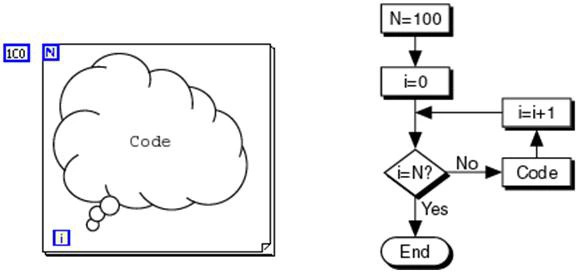
\includegraphics[width=.6\textwidth]{../../static/lw/for-cycle.jpeg}
  \caption{\tc{for} ciklus a LabView-ban}
  \label{fig:lw/for}
\end{figure}

\paragraph*{While Loop}
Ha az ismétlés közben derül ki, hogy kell-e még ismételni (például iteráció),
akkor \cix{while} ciklust használunk, amely egy hátul tesztelő ciklus.
\begin{figure}[H]
  \centering
  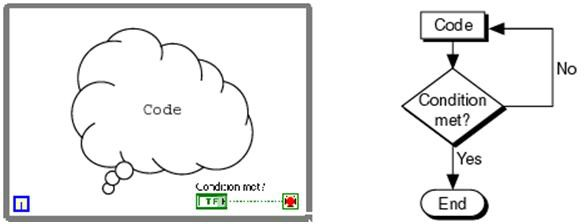
\includegraphics[width=.6\textwidth]{../../static/lw/while-loop.jpeg}
  \caption{\tc{while} ciklus a LabView-ban}
  \label{fig:lw/while}
\end{figure}

\paragraph*{Case Structure}
Az elágazásokat tipikusan \cix{case} struktúrákkal tudjuk kezelni.
A struktúrához tudunk esetet hozzáadni, diplikálni, vagy törölni.
Esetfeltételnek akár intervallumokat is megadhatunk:
\begin{figure}[htb]
  \centering
  \hfill
  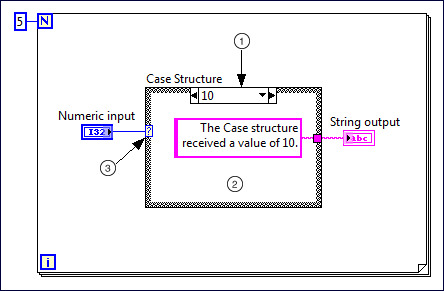
\includegraphics[height=3cm]{../../static/lw/case1.jpeg}
  \hfill
  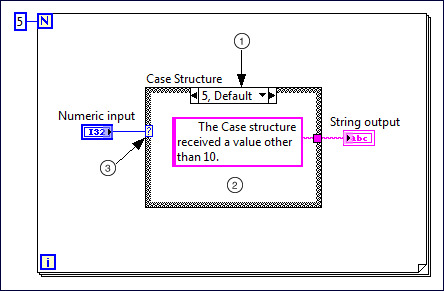
\includegraphics[height=3cm]{../../static/lw/case2.jpeg}
  \hfill
  \caption{\tc{case} struktúra LabView-ban}
  \label{fig:lw/case}
\end{figure}
\begin{itemize}
  \item \fbox{\texttt{1, 3, 5, 11}} -- a felsorolt értékek bármelyike,
  \item \fbox{\texttt{1..7}} -- a két érték közötti zárt intervallum,
  \item \fbox{\texttt{..7}} -- az érték és a nála nagyobb számok,
  \item \fbox{\texttt{7..}} -- az érték és a nála kisebb számok,
  \item \fbox{\texttt{1,2,4..7}} -- vegyesen.
\end{itemize}

\paragraph*{Formula Node}
Ebbe a keretbe, mint valami szövegszerkesztőbe lehet szöveges programkódot
írni. A Formula Node keretének szélén bárhol létrehozhatunk ún. terminálokat,
amelyeken keresztül kapcsolódik a grafikus és a szöveges programrész.
A kapcsolódás csak egyirányú lehet, vagy input (bemeneti), vagy output (kimeneti).
\begin{figure}[htb]
  \centering
  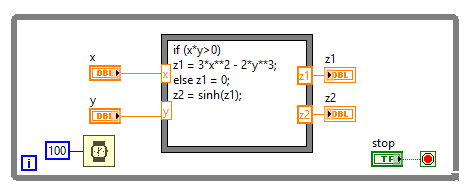
\includegraphics[width=.75\textwidth]{../../static/lw/fnode1.png}
  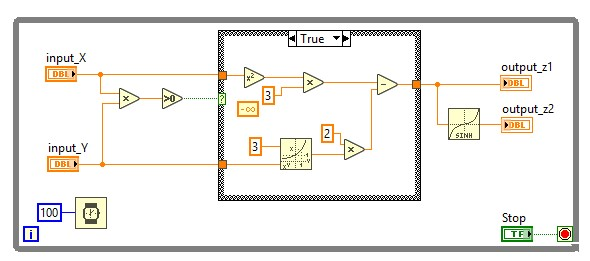
\includegraphics[width=.75\textwidth]{../../static/lw/fnode2.jpeg}
  \caption{Probléma megoldása \cix{Formula Node}-dal és nélküle}
  \label{fig:lw/fnode}
\end{figure}

\paragraph*{Flat Sequence}
A sorrendiség szabályozására való struktúra. A formáját a filmszalagtól
örökölte, utalva arra, hogy ahogyan a film esetén a kockák egymást követik,
itt is pontosan ez történik a végrehajtás során. A kockák egymás mellett
helyezkednek el, így egyszerre többet is láthatunk. A kockák közti
adatforgalom sem gond, mert egyszerűen áthúzzuk a vezetéket a határon.
\begin{figure}[htb]
  \centering
  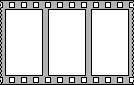
\includegraphics[width=.25\textwidth]{../../static/lw/fseq.jpeg}
  \caption{\cix{Flat Sequence} LabvView-ban}
  \label{fig:lw/fseq}
\end{figure}

\paragraph*{MathScript}
Nem kívánja meg a telepített MATLAB jelenlétét. Bemeneteket a \cix{Formula Node}-hoz
hasonlóan tudunk létrehozni, a keret bármely részén. A kimenetet viszont csak
a node-ban használt változókból csinálhatunk, és ezt addig nem engedi, amíg
létre nem hoztuk őket. Ekkor egy listából kell választanunk.


% \paragraph*{Local Variable}

% \paragraph*{Global Variable}

\end{document}
